\documentclass[12pt]{report} % You can also use 'article' or another class

% Import the geometry package to adjust margins
\usepackage[a4paper, margin=1in]{geometry} % Adjust margin as needed
\usepackage{fullpage}
\usepackage{wrapfig}
\usepackage{graphicx}
\usepackage[utf8]{inputenc}
\usepackage{multirow}
\usepackage[table]{xcolor}
\usepackage{color,soul}
\usepackage{chngcntr}
\usepackage{listings}
\usepackage{blindtext}
\usepackage{amsmath}
\usepackage{subfig} % Use this instead of subfigure
\usepackage{multicol}
\usepackage{adjustbox}
\usepackage{tabularx}  % For table resizing
\usepackage{float}     % For table placement
\usepackage{geometry}  % For page margin adjustments
\geometry{a4paper, margin=1in}
\usepackage{caption}   % For better table captions
\usepackage{booktabs}
\usepackage[hidelinks]{hyperref}
\usepackage{titlesec} % For section/chapter font customization
\usepackage{longtable}
\usepackage{lscape} % Use landscape for larger tables if needed

\definecolor{myblue}{RGB}{135,206,250}
\definecolor{dkgreen}{rgb}{0,0.6,0}
\definecolor{gray}{rgb}{0.5,0.5,0.5}
\definecolor{mauve}{rgb}{0.58,0,0.82}

\lstset{frame=tb,
  language=Python,
  aboveskip=3mm,
  belowskip=3mm,
  showstringspaces=false,
  columns=flexible,
  basicstyle={\small\ttfamily},
  numbers=none,
  numberstyle=\tiny\color{gray},
  keywordstyle=\color{blue},
  commentstyle=\color{dkgreen},
  stringstyle=\color{mauve},
  breaklines=true,
  breakatwhitespace=true,
  tabsize=3
}

\title{Pseudo Spectral Methods for Optimal Control}
\date{August 19, 2024}
\author{}

\begin{document}

\maketitle

\tableofcontents

\listoffigures

\chapter{Introduction}
Pseudo Spectral Methods for optimal control are a class of numerical techniques used for solving optimal control problems by approximating the state and control variables using spectral methods.

\section{Spectral Methods and Pseudospectral Methods}

\subsection{Spectral Methods}

\textbf{Definition}: Spectral methods are numerical techniques used for solving differential and integral equations by expanding the solution in terms of globally defined basis functions, such as orthogonal polynomials or trigonometric functions.

\subsubsection{Core Idea}
The core idea is to represent the solution \( u(x) \) as a series:
\[
u(x) \approx \sum_{n=0}^{N} a_n \phi_n(x),
\]
where \( \phi_n(x) \) are the chosen basis functions, and \( a_n \) are coefficients determined by projecting the original problem onto the basis functions.

\subsubsection{Types of Spectral Methods}
\begin{itemize}
    \item \textbf{Fourier Spectral Method}:
    \begin{itemize}
        \item \textbf{Basis Functions}: Trigonometric functions such as sine and cosine.
        \item \textbf{Application}: Best suited for problems with periodic boundary conditions.
        \item \textbf{Formulation}:
        \[
        u(x) \approx \sum_{k=-N/2}^{N/2} \hat{u}_k e^{ikx},
        \]
        where \( \hat{u}_k \) are the Fourier coefficients.
    \end{itemize}
    
    \item \textbf{Polynomial Spectral Method}:
    \begin{itemize}
        \item \textbf{Basis Functions}: Orthogonal polynomials, e.g., Chebyshev or Legendre polynomials.
        \item \textbf{Application}: Suitable for non-periodic boundary conditions.
        \item \textbf{Formulation}:
        \[
        u(x) \approx \sum_{n=0}^{N} a_n \phi_n(x),
        \]
        where \( a_n \) are coefficients found through projection.
    \end{itemize}
\end{itemize}

\subsubsection{Advantages and Disadvantages}
\begin{itemize}
    \item \textbf{Advantages}:
    \begin{itemize}
        \item High accuracy for smooth problems (exponential convergence).
        \item Efficient for global behavior of solutions.
    \end{itemize}
    \item \textbf{Disadvantages}:
    \begin{itemize}
        \item Not well-suited for non-smooth solutions.
        \item More complex for problems with sharp discontinuities.
    \end{itemize}
\end{itemize}

\subsection{Pseudospectral Methods}

\textbf{Definition}: Pseudospectral methods approximate derivatives and solve differential equations by evaluating the function at selected collocation points, instead of directly manipulating the coefficients in the basis function expansion.

\subsubsection{Core Idea}
The function \( u(x) \) is expanded similarly to spectral methods:
\[
u(x) \approx \sum_{n=0}^{N} a_n \phi_n(x).
\]
However, the derivatives are computed at discrete points, known as collocation points, leading to a practical discretization.

\subsubsection{Collocation Points}
Common choices for collocation points include:
\begin{itemize}
    \item \textbf{Chebyshev Nodes}:
    \[
    x_k = \cos\left(\frac{2k - 1}{2N} \pi\right), \quad k = 1, 2, \dots, N.
    \]
    \item \textbf{Gauss-Lobatto Points}: Nodes used for polynomial interpolation, chosen to enhance numerical stability and minimize errors.
\end{itemize}

\subsubsection{Types of Pseudospectral Methods}
\begin{itemize}
    \item \textbf{Fourier Pseudospectral Method}:
    \begin{itemize}
        \item Utilizes FFT for fast computation.
        \item Ideal for periodic problems.
    \end{itemize}
    
    \item \textbf{Chebyshev Pseudospectral Method}:
    \begin{itemize}
        \item Uses Chebyshev polynomials and their nodes for derivatives.
        \item Suitable for non-periodic problems.
    \end{itemize}
\end{itemize}

\subsubsection{Formulation}
For a function \( u(x) \) and its derivative \( u'(x) \), the derivative at collocation points \( x_k \) can be approximated as:
\[
u'(x_k) \approx \sum_{j=0}^{N} D_{kj} u(x_j),
\]
where \( D_{kj} \) is the differentiation matrix based on the basis functions.

\subsubsection{Advantages and Disadvantages}
\begin{itemize}
    \item \textbf{Advantages}:
    \begin{itemize}
        \item Flexible for complex boundary conditions.
        \item High accuracy, similar to spectral methods, with a practical approach to discretization.
    \end{itemize}
    \item \textbf{Disadvantages}:
    \begin{itemize}
        \item Computational cost due to dense matrix operations.
        \item Sensitive to the choice of collocation points.
    \end{itemize}
\end{itemize}

\subsection{Comparison Between Spectral and Pseudospectral Methods}
\begin{itemize}
    \item \textbf{Approach to Differentiation}:
    \begin{itemize}
        \item \textbf{Spectral Methods}: Operate in the spectral space by manipulating expansion coefficients.
        \item \textbf{Pseudospectral Methods}: Operate in the physical space by evaluating derivatives at collocation points.
    \end{itemize}
    
    \item \textbf{Flexibility}:
    \begin{itemize}
        \item \textbf{Spectral Methods}: Less flexible for complex boundaries.
        \item \textbf{Pseudospectral Methods}: More adaptable for varied boundary conditions.
    \end{itemize}
    
    \item \textbf{Implementation}:
    \begin{itemize}
        \item \textbf{Spectral Methods}: Require exact integration for coefficient projection.
        \item \textbf{Pseudospectral Methods}: Use discrete points and fast algorithms like FFT.
    \end{itemize}
\end{itemize}


\section{Introduction}
Pseudospectral methods are a class of numerical techniques used primarily for solving differential equations, particularly in the context of optimal control problems and partial differential equations. They combine the strengths of spectral methods and finite difference methods. Spectral methods approximate the solution to a differential equation by expressing it as a sum of global basis functions, typically orthogonal polynomials like Chebyshev polynomials or trigonometric functions. Pseudospectral methods are a specific type of spectral method where the differential equation is enforced at a set of discrete points in the domain, known as collocation points.

The concepts of direct and indirect methods are widely used in optimal control theory and numerical optimization. The two approaches differ fundamentally in the sequence in which they handle the discretization and optimization processes. In direct methods, the problem is first discretized and then optimized.

In this course, we will be using direct methods with a major focus on the discretization part.

\section{Important Terms}
Brief introduction to the important terms we will be using in the discussions.

\subsection{Optimal Control Problem}
Components of an Optimal Control Problem:
\begin{enumerate}
    \item \textbf{State Variables} \(x(t)\): These describe the state of the system at any time \(t\). The evolution of these states is typically governed by differential equations.
    \item \textbf{Control Variables} \(u(t)\): These are the inputs or decisions that can be manipulated over time to influence the behavior of the state variables.
    \item \textbf{Dynamics (State Equations)}:
    \[
    \dot{x}(t) = f(x(t), u(t), t)
    \]
    This is a set of differential equations describing how the state variables evolve over time as a function of the current state, control inputs, and time.
    \item \textbf{Cost Function (Objective Function)}:
    \[
    J = \int_{t_0}^{t_f} L(x(t), u(t), t)\, dt + \Phi(x(t_f))
    \]
    Here, \(L(x(t), u(t), t)\) is the running cost (instantaneous cost rate), and \(\Phi(x(t_f))\) is the terminal cost at the final time \(t_f\). The goal is to minimize (or maximize) this cost function.
    \item \textbf{Boundary Conditions}:
    \[
    x(t_0) = x_0 \quad \text{and possibly} \quad x(t_f) = x_f
    \]
    These specify the initial state (and sometimes the final state) of the system.
    \item \textbf{Constraints}: These can include state constraints, control constraints, and mixed constraints.
    \begin{itemize}
        \item \textbf{State Constraints}: \(g(x(t)) \leq 0\)
        \item \textbf{Control Constraints}: \(h(u(t)) \leq 0\)
        \item \textbf{Mixed Constraints}: Involving both state and control variables.
    \end{itemize}
\end{enumerate}


\section{Least Squares Approach}
The \textbf{Least Squares approach} is a mathematical method used to find the best-fitting solution to a set of data by minimizing the sum of the squares of the differences between the observed and predicted values. Suppose you have a set of observed data points $(x_i, y_i)$, and you want to fit a model $f(x)$ to these data points. The least squares method minimizes the following sum:

\begin{equation}
    S = \sum_{i=1}^{n} \left( y_i - f(x_i) \right)^2
\end{equation}

In the least squares method, the approximated function is not guaranteed to be equal to the value of the actual function at the node points.

\section{Interpolation}
\textbf{Interpolation} is a mathematical technique used to estimate unknown values that fall within the range of known data points. It is widely used in numerical analysis, data science, engineering, and other fields where it is necessary to predict values for intermediate points based on a set of discrete data points. Unlike the least squares approach, in interpolation, the modeled function passes through the selected data points.

One common interpolation method is the \textbf{Lagrange Interpolation}, which constructs the interpolating polynomial using a linear combination of Lagrange basis polynomials. The interpolating polynomial $P(x)$ is given by:

\begin{equation}
    P(x) = \sum_{i=0}^{n} y_i \prod_{\substack{0 \leq j \leq n \\ j \neq i}} \frac{x - x_j}{x_i - x_j}
\end{equation}

\section{Class Discussion - MATLAB Plot: Least Squares vs Interpolation}
As discussed in class, the interpolation method ensures that the value of the approximated function is exactly the value of the actual function at the selected node points. Figure \ref{fig:comparison_plot} shows the difference between the two approximation methods (Least Squares and Interpolation) via a simple MATLAB plot discussed during the lecture.

\begin{figure}[h]
    \centering
    \includegraphics[width=0.7\textwidth]{least_squares_vs_interpolation.png} % Include your plot here
    \caption{Comparison of Least Squares and Interpolation Methods.}
    \label{fig:comparison_plot}
\end{figure}

\section{Collocation Method}
The collocation method is a technique used to approximate solutions of differential equations by forcing the solution to satisfy the differential equation at a finite number of points called collocation points.
For a given set of nodes, the polynomial can be approximated in either of the two ways:

\begin{equation}
    P_n(x) = \sum_{i=0}^{n} a_i f(x_i)
\end{equation}

or

\begin{equation}
    P_n(x) = \sum_{i=0}^{n} b_i x_i
\end{equation}

Both of these are types of interpolation matrices, and the value of the approximated polynomial is the same as the actual function at the node points.

\subsection{Vandermonde Matrix}
Given a vector of elements \( x = [x_1, x_2, \dots, x_n] \), the Vandermonde matrix \( V \) associated with this vector is an \( n \times n \) matrix, where each row corresponds to a geometric progression of the elements \( x_i \). Specifically, the matrix is defined as follows:

\[
V = \begin{pmatrix}
    1 & x_1 & x_1^2 & \dots & x_1^{n-1} \\
    1 & x_2 & x_2^2 & \dots & x_2^{n-1} \\
    \vdots & \vdots & \vdots & \dots & \vdots \\
    1 & x_n & x_n^2 & \dots & x_n^{n-1} 
\end{pmatrix}
\]

Each element \( V_{ij} \) in the matrix is given by:

\begin{equation}
    V_{ij} = x_i^{j-1}
\end{equation}

The determinant of the Vandermonde matrix has a special form and is given by:

\begin{equation}
    \det(V) = \prod_{1 \leq i < j \leq n} (x_j - x_i)
\end{equation}

This product is non-zero if and only if all the \( x_i \) are distinct, meaning the determinant of the Vandermonde matrix is non-zero (and hence the matrix is invertible) if all the elements in the vector \( x \) are distinct. The proof for this will be discussed later.

\section{Runge Phenomenon}
When interpolating a set of points, one common approach is to fit a polynomial that passes through all the given data points. The idea is that the polynomial will closely approximate the underlying function from which the data points are sampled. However, when the function is sampled at equally spaced points and a high-degree polynomial is used, the interpolation error can become quite significant near the endpoints of the interval. This is known as \textbf{Runge's Phenomenon}.

\section{Chebyshev Nodes}
Chebyshev nodes are specific points used in numerical interpolation, particularly in polynomial interpolation, to reduce the problems associated with Runge's phenomenon and to achieve more accurate approximations.\\\\
Chebyshev nodes are the roots of Chebyshev polynomials of the first kind. For a given interval \([-1, 1]\), the Chebyshev nodes \(x_i\) for \(n\) interpolation points are defined as:
\begin{equation}
    x_i = \cos\left(\frac{2i - 1}{2n} \pi\right), \quad i = 1, 2, \dots, n
\end{equation}
These nodes are spaced more densely near the endpoints of the interval \([-1, 1]\) and more sparsely near the center. When interpolating over a different interval \([a, b]\), you can linearly transform the Chebyshev nodes from \([-1, 1]\) to \([a, b]\) using the transformation:
\[
x'_i = \frac{b-a}{2} \left( x_i + 1 \right) + a
\]

\section{Weierstrass Theorem}
The \textbf{Weierstrass Approximation Theorem} states that for every continuous function \(f\) defined on a closed interval \([a, b]\), and for every \(\epsilon > 0\), there exists a polynomial \(P(x)\) such that:

\begin{equation}
    \|f(x) - P(x)\| < \epsilon
\end{equation}

for all \(x\) in \([a, b]\). In other words, any continuous function on a closed interval can be uniformly approximated as closely as desired by a polynomial function. The proof of the Weierstrass Approximation Theorem typically involves constructing a sequence of polynomials that converge uniformly to the given continuous function. One standard approach uses Bernstein polynomials, which are constructed from binomial coefficients and shown to converge uniformly to the function \(f(x)\).

\section{Trapezoidal Method}
The \textbf{Trapezoidal Method} is used to approximate the area under a curve by dividing the region into a series of trapezoids. The area of each trapezoid is computed and summed to give an approximation of the definite integral.

Consider a function \(f(x)\) defined on the interval \([a, b]\). The goal is to approximate the definite integral:

\begin{equation}
    \int_a^b f(x) dx
\end{equation}

Using the trapezoidal method, the interval \([a, b]\) is divided into \(n\) subintervals of equal width:

\[
h = \frac{b - a}{n}
\]

The points dividing the interval are:

\[
x_0 = a, \quad x_1 = a + h, \quad x_2 = a + 2h, \dots, x_n = b
\]

The trapezoidal rule then approximates the integral as:

\begin{equation}
    \int_a^b f(x) dx \approx \frac{h}{2} \left[ f(x_0) + 2f(x_1) + 2f(x_2) + \dots + 2f(x_{n-1}) + f(x_n) \right]
\end{equation}

This formula sums the function values at the endpoints and the midpoints, weighted appropriately, to give a numerical estimate of the integral.

\section{Trapezoidal Method}
\subsection{Example}
The Trapezoidal method provides good accuracy for periodic functions and becomes exact after a certain number of nodes are used for discretization. (The proof for this can be found in the class notes on Moodle.) Figure \ref{fig:trapezoid_accuracy} demonstrates the accuracy of the trapezoidal method, as shown by the MATLAB code discussed in class.

\begin{figure}[h!]
    \centering
    \includegraphics[width=0.8\textwidth]{trapezoid_accuracy.png} % Assuming you have an image here.
    \caption{Trapezoid method accuracy.}
    \label{fig:trapezoid_accuracy}
\end{figure}

\section{Central Difference Method}
The Central Difference method is a finite difference scheme used to approximate derivatives by expanding around two neighboring points. It is second-order accurate, meaning it approximates derivatives to second-order accuracy in terms of the grid spacing \(\Delta x\).

\subsection{Expansion Around \(x_{i+1} = x_i + \Delta x\)}
By expanding the function \(f(x)\) around \(x_{i+1} = x_i + \Delta x\), we obtain the following Taylor series expansion:

\begin{equation}
    f(x_{i+1}) = f(x_i + \Delta x) = f(x_i) + \frac{f'(x_i)}{1!} \Delta x + \frac{f''(x_i)}{2!} (\Delta x)^2 + \frac{f'''(x_i)}{3!} (\Delta x)^3 + O((\Delta x)^4)
\end{equation}

\subsection{Expansion Around \(x_{i-1} = x_i - \Delta x\)}
Similarly, expanding the function around \(x_{i-1} = x_i - \Delta x\), we get:

\begin{equation}
    f(x_{i-1}) = f(x_i - \Delta x) = f(x_i) - \frac{f'(x_i)}{1!} \Delta x + \frac{f''(x_i)}{2!} (\Delta x)^2 - \frac{f'''(x_i)}{3!} (\Delta x)^3 + O((\Delta x)^4)
\end{equation}

\subsection{Central Difference Formula}
Taking the difference between \(f(x_{i+1})\) and \(f(x_{i-1})\), we get:

\begin{equation}
    f(x_{i+1}) - f(x_{i-1}) = 2 f'(x_i) \Delta x + \frac{2 f'''(x_i)}{6} (\Delta x)^3 + O((\Delta x)^4)
\end{equation}

Approximating over small intervals, the first derivative \(f'(x_i)\) is approximated as:

\begin{equation}
    f'(x_i) \approx \frac{f(x_{i+1}) - f(x_{i-1})}{2\Delta x}
\end{equation}

Thus, the central difference scheme provides exact results if the highest order of the function is cubic.

\subsection{Higher-Order Central Difference}
By increasing the size of the stencil (i.e., including more neighboring points), we can reduce the approximation error and improve the accuracy of the method. As the stencil size increases, the error tends toward zero for higher-order functions.

\section{Example Problem}
Consider a block with the following boundary conditions:

\[
x(0) = 0, \quad v(0) = 0, \quad x(1) = 1, \quad v(1) = 0
\]

The system is governed by the equations:

\[
\dot{x} = v, \quad \dot{v} = u
\]

The objective is to optimize the following function:

\[
J = \int_0^1 U(x)^2 \, dx
\]

Using the trapezoidal method, we can approximate the integral as:

\[
J = \left( \frac{U_0^2}{2} + U_1^2 + \cdots + U_{n-1}^2 + \frac{U_n^2}{2} \right) \Delta t
\]

### Two Methods for Non-Linear Equality Constraints:

#### 1. Central Difference Method
In the central difference method, the constraint conditions are formed as follows for the interior points:

\[
\frac{x_{k+1} - x_{k-1}}{2h} = v_k, \quad \frac{v_{k+1} - v_{k-1}}{2h} = u_k
\]

For the boundary points, forward and backward Euler methods are used to satisfy the conditions at the boundaries.

#### 2. Trapezoidal Method
In the trapezoidal method, the constraint conditions are written as:

\[
x_{k+1} - x_k = \frac{v_{k+1} + v_k}{2} \Delta t, \quad v_{k+1} - v_k = \frac{u_{k+1} + u_k}{2} \Delta t
\]

The full implementation of this method can be found in the \texttt{nonlincon.m} file, as discussed in class.

To perform the optimization, we use the \texttt{fmincon} function from MATLAB. \texttt{fmincon} is used for solving constrained nonlinear optimization problems, and it finds the minimum of a scalar function subject to the specified constraints.

\section{Discussion of MATLAB and Mathematica Presentation in Class}
With the same boundary conditions as the previous problem, a related problem discussed in class has 5 unknowns and 4 conditions, making it an optimization problem. This requires the use of similar numerical methods for solution.

\section{Rolle's Theorem}
Rolle’s Theorem is a fundamental result in calculus that provides a specific condition under which a function must have a horizontal tangent line (or a derivative equal to zero) at least once within a given interval.

The theorem states that if a continuous function \(f(x)\) is differentiable on the open interval \((a, b)\) and satisfies \(f(a) = f(b)\), then there exists at least one point \(c \in (a, b)\) such that:

\[
f'(c) = 0
\]

This result is often used in optimization and root-finding algorithms.

\section{Rolle's Theorem}
Rolle’s Theorem is a fundamental result in calculus that provides a specific condition under which a function must have a horizontal tangent line (or a derivative equal to zero) at least once within a given interval. It’s a special case of the Mean Value Theorem.

Let \( f(x) \) be a function that satisfies the following three conditions:
\begin{enumerate}
    \item \textbf{Continuity:} \( f(x) \) is continuous on the closed interval \([a, b]\).
    \item \textbf{Differentiability:} \( f(x) \) is differentiable on the open interval \((a, b)\).
    \item \textbf{Equal Endpoints:} \( f(a) = f(b) \).
\end{enumerate}

If these conditions are met, then there exists at least one point \( c \in (a, b) \) such that the derivative of \( f(x) \) at \( c \) is zero:

\[
f'(c) = 0
\]

\section{Derivatives of Lagrange Polynomial}
Consider a function approximated with a second-order Lagrange polynomial using equally spaced nodes at \(0\), \(h\), and \(2h\). The polynomial can be expressed as:

\[
P(x) = y_0 \cdot \ell_0(x) + y_1 \cdot \ell_1(x) + y_2 \cdot \ell_2(x)
\]

Where the Lagrange basis polynomials are defined as follows:

\[
\ell_0(x) = \frac{(x - x_1)(x - x_2)}{(x_0 - x_1)(x_0 - x_2)}
\]

\[
\ell_1(x) = \frac{(x - x_0)(x - x_2)}{(x_1 - x_0)(x_1 - x_2)}
\]

\[
\ell_2(x) = \frac{(x - x_0)(x - x_1)}{(x_2 - x_0)(x_2 - x_1)}
\]

The derivative of the polynomial \( P'(x) \) is given by:

\[
P'(x) = y_0 \cdot \frac{2x - (x_1 + x_2)}{(x_0 - x_1)(x_0 - x_2)} + y_1 \cdot \frac{2x - (x_0 + x_2)}{(x_1 - x_0)(x_1 - x_2)} + y_2 \cdot \frac{2x - (x_0 + x_1)}{(x_2 - x_0)(x_2 - x_1)}
\]

To represent the derivatives at the node points in matrix format, we can express it as:

\[
\begin{bmatrix}
P'(x_0) \\
P'(x_1) \\
P'(x_2)
\end{bmatrix} =
\begin{bmatrix}
-\frac{3}{2h} & \frac{2}{h} & -\frac{1}{2h} \\
-\frac{1}{2h} & 0 & \frac{1}{h} \\
\frac{1}{h} & -\frac{2}{h} & \frac{3}{2h}
\end{bmatrix}
\begin{bmatrix}
P(x_0) \\
P(x_1) \\
P(x_2)
\end{bmatrix}
\]

This shows that the derivatives of the approximated function at the node points are a linear combination of the actual function values at the node points.

\section{Controlling Error by Altering the Location of Nodes}
\textbf{Claim:} When we approximate a function using a polynomial of order \( n \), the error in the representation can be altered by changing the position of the nodes (collocation points).\\\\
\textbf{Proof:} Consider the error term defined as:
\[
W(t) = f(t) - p_n(f; t) - (t - x_0)(t - x_1) \cdots (t - x_n) K(x)
\]
Where \( K(x) \) is defined as:
\[
K(x) = \frac{f(x) - p_n(f; x)}{(x - x_0)(x - x_1) \cdots (x - x_n)}
\]
For an \( n \)-th order polynomial, we have \( (n + 1) \) variables. The function \( W \) is zero at:
\begin{itemize}
    \item \( t = x_i \) for all \( i = 0, 1, \ldots, n \) (the node points)
    \item \( t = x \)
\end{itemize}

By applying Rolle’s Theorem, there exists some \( \xi \) in the interval between \( x_0 \) and \( x_n \) such that:
\[
W^{(n+1)}(t) = f^{(n+1)}(t) - (n + 1)! K(x)
\]
Thus, at point \( \xi \):
\[
0 = W^{(n+1)}(\xi) = f^{(n+1)}(\xi) - (n + 1)! K(x)
\]
From this, we can express \( K(x) \) as:
\[
K(x) = \frac{1}{(n + 1)!} f^{(n+1)}(\xi)
\]
Consequently, the error \( e(x) \) can be written as:
\[
e(x) = f(x) - p_n(x) = \frac{1}{(n + 1)!} f^{(n+1)}(\xi) (x - x_0)(x - x_1) \cdots (x - x_n)
\]
This shows that while we do not have direct control over \( f^{(n+1)} \) to reduce the error, we can alter the location of the nodes to change the error. \\\\
Figure 4 shows the class representation in Mathematica, illustrating that for a function approximated using a second-order polynomial, taking the derivative at the central control point is the same as applying the central difference at that point.

\section{Difference Between a Polynomial and Its \( n \)th Order Interpolation Approximation}
The error in approximating a function \( f(x) \) using an \( n \)th order polynomial \( p_n(x) \) can be expressed as:

\[
e(x) = f(x) - p_n(x) = \frac{1}{(n + 1)!} f^{(n+1)}(\xi)(x - x_0)(x - x_1) \cdots (x - x_n)
\]

From MATLAB simulations, we found that the optimal node locations for approximating a 2D polynomial with a linear Lagrange polynomial (in the symmetric case) are as follows:
- For least RMS error: \( x_0 = -\sqrt{\frac{1}{3}} \) and \( x_1 = \sqrt{\frac{1}{3}} \)
- For least maximum error: \( x_0 = -\sqrt{\frac{1}{2}} \) and \( x_1 = \sqrt{\frac{1}{2}} \)

Figure 5 shows the Mathematica representation of these findings as discussed in class. A similar analysis applies to a 3D polynomial; refer to the MATLAB code for the optimal node points for a third-order polynomial function.

\section*{Example Problem}
Consider a polynomial function \( X_{n+1} \) represented using an \( n \)th order polynomial:

\[
P_n = \sum_{i=0}^{n} a_i x^i
\]

We need to find the leading coefficient of the approximation, \( a_n \). Equally spaced node points are chosen from 0 to 1 (including both endpoints).

\textbf{Solution:} Using the remainder theorem:

\[
X_{n+1} - \sum_{i=0}^{n} a_i x^i = A (x - 0)(x - \frac{1}{n})(x - \frac{2}{n}) \cdots (x - \frac{n-1}{n})(x - 1)
\]

Here, \( A \) comes out to be 1. Comparing the coefficients on the left-hand side and the right-hand side, we find the leading coefficient \( a_n = \frac{n + 1}{2} \).

\section{Condition for Vandermonde Matrix Being Invertible}
The Vandermonde matrix is always invertible except when two node points are the same. To understand this, we can observe the Vandermonde matrix defined as:

\[
V =
\begin{pmatrix}
1 & x_0 & x_0^2 & \cdots & x_0^n \\
1 & x_1 & x_1^2 & \cdots & x_1^n \\
\vdots & \vdots & \vdots & \ddots & \vdots \\
1 & x_n & x_n^2 & \cdots & x_n^n
\end{pmatrix}
\]

If two node points become the same, two rows of the matrix become identical, causing the determinant to be zero, thus making the matrix non-invertible.

Now, consider the Vandermonde matrix with the last row replaced by \( x \) instead of \( x_n \):

\[
V =
\begin{pmatrix}
1 & x_0 & x_0^2 & \cdots & x_0^n \\
1 & x_1 & x_1^2 & \cdots & x_1^n \\
\vdots & \vdots & \vdots & \ddots & \vdots \\
1 & x & x^2 & \cdots & x^n
\end{pmatrix}
\]

If \( x \) takes any of the values \( x_0, x_1, \ldots, x_{n-1} \), the determinant is zero. Thus, the determinant can be expressed as:

\[
\text{det}(V) = A \prod_{k=0}^{n-1} (x_n - x_k)
\]

Where \( A \) is a coefficient that does not contain any \( x \) term. Further observation shows that \( A \) is the determinant of a Vandermonde matrix with \( n \) terms, applying similar operations to \( x_n \) for \( x_{n-1} \) now:

\[
\text{det}(V) = (x_1 - x_0) \prod_{k=0}^{1} (x_2 - x_k) \prod_{k=0}^{2} (x_3 - x_k) \cdots \prod_{k=0}^{n-1} (x_n - x_k)
\]

This form proves that unless two nodes are identical, the determinant of the Vandermonde matrix will exist.

\section{Lagrange Basis Polynomial}

\subsection{Cramer’s Rule}
Consider a system of linear equations:

\[
Ax = b
\]

where:
- \( A \) is an \( n \times n \) matrix of coefficients,
- \( x \) is a column vector of unknowns,
- \( b \) is a column vector of constants.

Cramer’s Rule states that if \( \det(A) \neq 0 \), the solution to the system is given by:

\[
x_i = \frac{\det(A_i)}{\det(A)} \quad \text{for } i = 1, 2, \ldots, n,
\]

where \( A_i \) is obtained by replacing the \( i \)-th column of \( A \) with \( b \).

\subsubsection{Proof}
For a particular \( m \), consider:

\[
x_m = \sum_{j=0}^{n} W(x_j)x_{j,m}
\]

where \( 0 \leq m \leq n \). Note that even though for all \( m \) less than \( n \), it appears that the right-hand side will have a higher power of \( x \) than \( m \) due to the Lagrange polynomial bases, the terms cancel out to match the power on the left-hand side.

The aim is to prove that 

\[
P_n(x) = \sum_{i=0}^{n} a_ix^i
\]

can be represented as 

\[
P_n(x) = \sum_{i=0}^{n} W_i f(x_i)
\]

where the \( W_i \) are the Lagrange bases.

Thus,

\[
P_n(x) = \sum_{k=0}^{n} a_k(x_k)
\]

can be rearranged as follows:

\[
P_n(x) = \sum_{k=0}^{n} a_k \sum_{j=0}^{n} W(x_j)x^j_k
\]

Rearranging gives:

\[
P_n(x) = \sum_{j=0}^{n} W(x_j) \sum_{k=0}^{n} a_k x_j^k
\]

Therefore,

\[
P_n(x) = \sum_{j=0}^{n} W(x_j) P(x_j)
\]

To find the Lagrange basis, we write the system of equations in a matrix format:

\[
\begin{pmatrix}
1 & 1 & \cdots & 1 \\
x_1 & x_2 & \cdots & x_n \\
x_1^2 & x_2^2 & \cdots & x_n^2 \\
\vdots & \vdots & \ddots & \vdots \\
x_{n-1} & 1 & x_{n-1}^2 & \cdots & x_{n-1}^n
\end{pmatrix}
\begin{pmatrix}
W_0 \\
W_1 \\
W_2 \\
\vdots \\
W_n
\end{pmatrix}
=
\begin{pmatrix}
x_0 \\
x_1 \\
x_2 \\
\vdots \\
x_n
\end{pmatrix}
\]

Notably, the Vandermonde matrix \( V \) is given by:

\[
V^T =
\begin{pmatrix}
1 & 1 & \cdots & 1 \\
x_1 & x_2 & \cdots & x_n \\
x_1^2 & x_2^2 & \cdots & x_n^2 \\
\vdots & \vdots & \ddots & \vdots \\
x_{n-1} & 1 & x_{n-1}^2 & \cdots & x_{n-1}^n
\end{pmatrix}
\]

Using Cramer’s rule, we know that:

\[
W_j = \frac{\Delta_j}{\Delta}
\]

where \( \Delta \) is the determinant of the Vandermonde matrix and \( \Delta_j \) is the determinant of the Vandermonde matrix with the elements \( x_j \) replaced with \( x \).

To find the Lagrange polynomials:

\[
\Delta = \det(V) = (x_1 - x_0) \prod_{k=1}^{n-1} (x_2 - x_k) \prod_{k=2}^{n-1} (x_3 - x_k) \cdots \prod_{k=n-1}^{n-1} (x_n - x_k)
\]

Separating all terms that have an \( x_j \) in them:

\[
\det(V) = \lambda_j \prod_{k=0}^{j-1} (x_j - x_k) \prod_{k=j+1}^{n} (x_k - x_j)
\]

Here, \( \lambda_j \) is the part of the determinant that does not have any \( x_j \) terms. Replacing \( x_j \) with \( x \):

\[
\Delta_j = \det(V) = \lambda_j \prod_{k=0}^{j-1} (x - x_k) \prod_{k=j+1}^{n} (x_k - x)
\]

Thus,

\[
W(x_j) = \ell_j(x) = \prod_{\substack{0 \leq k \leq n \\ k \neq j}} \frac{x - x_k}{x_j - x_k}
\]

We can conclude that all the Lagrange basis polynomials are of the same order, and for \( n + 1 \) node points over which the polynomial is approximated, the basis function will be of order \( n \). Note that the Lagrange basis polynomial \( \ell_j \) has a value of 1 at the node \( x_j \) and zero at all other node points. The polynomial cannot have more zeros than the number of remaining node points, as verified from the degree of the polynomial.

\subsection{Important Points}

\subsubsection{Intuitive Understanding of Why the Sum of Weights is One}
Every approximation of a function must be able to model a constant function as well. Thus, the sum of weights or the coefficients must equal one. This can be mathematically represented as:

\[
P(x) = \sum_{i=0}^{n} W_k(x) f(x_k)
\]

For a constant function, say \( f(x) = c \):

\[
P(x) = c = \sum_{i=0}^{n} W_k(x) c
\]

Canceling \( c \) on both sides gives:

\[
\sum_{i=0}^{n} W_k(x) = 1
\]


\section{Derivatives of Lagrange Polynomial/ Differentiation Matrix}
The derivative of a Lagrange polynomial can be computed using specific formulas, which are essential in interpolation problems.


\chapter{Runge Phenomena}
The Runge phenomenon refers to the large oscillations that can occur when using polynomial interpolation at equidistant points.

\section{Controlling error by controlling location of nodes}
By strategically choosing the locations of interpolation nodes, one can minimize the error in polynomial interpolation.

\section{Chebyshev Nodes}
Chebyshev nodes are specific points used in polynomial interpolation to minimize the interpolation error, particularly to avoid the Runge phenomenon.

\chapter{Weistress Theorem}
The Weistress approximation theorem states that any continuous function defined on a closed interval can be uniformly approximated by polynomial functions to any degree of accuracy.

\section*{Weierstrass Theorem (Bernstein polynomial)}

\[
\exists \ P_n(x) \text{ such that } |f(x) - P_n(x)| < \epsilon
\]
\[
f(x), \ x \in [0, 1]
\]
\[
|f(x) - f(x_0)| < \epsilon
\]
\[
x \in [x_0 - \delta, x_0 + \delta] \quad \text{closed interval (can go to $\infty$ at endpoints)}
\]
\[
(a + b)^n = \sum_{k=0}^{n} \binom{n}{k} a^{k} b^{n-k}
\]
\[
(a + (1 - x))^n = \sum_{k=0}^{n} \binom{n}{k} x^k (1 - x)^{n-k} = 1
\]
Bernstein polynomial terms: $B_k(x)$
\[
B_n(f, x) = \sum_{k=0}^{n} f\left( \frac{k}{n} \right) b_k(x)
\]
\[
\Rightarrow B_n(f) \to f
\]
\[
\left| B_n(f, x) - f(x) \right| = \left| \sum_{k=0}^{n} \left( f\left( \frac{k}{n} \right) - f(x) \right) b_k(x) \right|
\]
Trying to find upper bound for this
\[
|x - \frac{k}{n}| \leq \delta
\]

\[
f(x) \leq M \quad \text{bounded and continuous in interval taken}
\]

\[
|f(x) - f(x_0)| \leq 2M
\]
\section*{Further Analysis on Bernstein Polynomials}

\[
\left| \sum_{k=0}^{n} \left( f\left( \frac{k}{n} \right) - f(x) \right) b_k(x) \right| = \sum_{k=0}^{n} \left| f\left( \frac{k}{n} \right) - f(x) \right| b_k(x)
\]

\[
|B_n(f, x) - f(x)| \leq \sum_{|x - \frac{k}{n}| \leq \delta} \left| f\left( \frac{k}{n} \right) - f(x) \right| b_k(x) + \sum_{|x - \frac{k}{n}| > \delta} \left| f\left( \frac{k}{n} \right) - f(x) \right| b_k(x)
\]

\[
\leq \sum_{|x - \frac{k}{n}| \leq \delta} \frac{\epsilon}{2} b_k(x) + \sum_{|x - \frac{k}{n}| > \delta} \frac{2M}{n \delta^2} b_k(x)
\]

\[
\leq \sum_{|x - \frac{k}{n}| \leq \delta} \frac{\epsilon}{2} b_k(x) + \sum_{|x - \frac{k}{n}| > \delta} \frac{2M}{n \delta^2} b_k(x)
\]

Using bounds and conditions, we proceed as follows:

\[
= \sum_{|x - \frac{k}{n}| \leq \delta} \frac{\epsilon}{2} b_k(x) + \frac{2M}{n \delta^2} \sum_{|x - \frac{k}{n}| > \delta} b_k(x)
\]

Expanding on this:

\[
= \frac{\epsilon}{2} \sum b_k(x) + \frac{2M}{n \delta^2} \sum \left( \frac{k}{n} - x \right)^2 b_k(x)
\]

Define parameters for probability and expectation:
\[
p = nx, \quad \sigma = \sqrt{n x (1 - x)}, \quad E[(k - \mu)^2] = \sigma^2 = E[k^2] - E[k]^2
\]

\[
E[k] = \sum k \cdot p(k), \quad \sigma^2 = E[(k - \mu)^2]
\]

Where:
\[
E[(k - \mu)^2] = E[k^2] - E[k]^2 \quad \text{with} \quad \mu = nx
\]

\[
B_n(f, x) = \sum_{k=0}^{n} f\left( \frac{k}{n} \right) \binom{n}{k} x^k (1 - x)^{n-k}
\]

\[
|B_n(f, x) - f(x)| = \left| \sum_{k=0}^{n} \left( f\left( \frac{k}{n} \right) - f(x) \right) \binom{n}{k} x^k (1 - x)^{n-k} \right|
\]

\[
\leq \sum \left| f\left( \frac{k}{n} \right) - f(x) \right| \binom{n}{k} x^k (1 - x)^{n-k}
\]

\[
= \sum_{|x - \frac{k}{n}| \leq \delta} \left| f\left( \frac{k}{n} \right) - f(x) \right| \binom{n}{k} x^k (1 - x)^{n-k} + \sum_{|x - \frac{k}{n}| > \delta} \left| f\left( \frac{k}{n} \right) - f(x) \right| \binom{n}{k} x^k (1 - x)^{n-k}
\]

Define these two regions as:
\[
A = \sum_{|x - \frac{k}{n}| \leq \delta} \left| f\left( \frac{k}{n} \right) - f(x) \right| \binom{n}{k} x^k (1 - x)^{n-k} \leq \frac{\epsilon}{2}
\]

\[
B = \sum_{|x - \frac{k}{n}| > \delta} \left| f\left( \frac{k}{n} \right) - f(x) \right| \binom{n}{k} x^k (1 - x)^{n-k} 
\]

For \( B \):
\[
\leq \sum_{k \in B} \frac{2M}{n^2 \delta^2} \binom{n}{k} x^k (1 - x)^{n-k}
\]

Using the probability statistics:
\[
\leq \frac{\epsilon}{2} + \frac{2M}{n \delta^2}
\]

We adjust so that:
\[
\frac{M}{2n\delta} = \frac{\epsilon}{2} \Rightarrow \epsilon
\]

Thus:
\[
|B_n(f, x) - f(x)| \leq \epsilon
\]

Hence, this justifies that interpolation is valid.

\[
\int_0^1 h(t) \, dt
\]

And constraints:
\[
\mathbf{D} \mathbf{x} = A
\]


\[
\int_{0}^{T} h(t) \, dt \approx \int_{0}^{T} \sum_{k=0}^{n} h(t_k) L_k(t) \, dt 
= \sum_{k=0}^{n} h(t_k) \underbrace{\int_{0}^{T} L_k(t) \, dt}_{w_k}
\]
\[
h \in \mathbb{P}_n
\]

\noindent
{\textit{can this also be reversed}} \hspace{3cm}
{\textit{we're approximating the integral to a higher order to make it exact,}} \\
{\textit{not approximating the function.}}

\section{Bernstein Polynomials and Their Applications}

\textbf{Definition}: Bernstein polynomials are a particular set of polynomials that are used to approximate continuous functions on a closed interval \( [0, 1] \). They are fundamental in approximation theory and are used to prove the Weierstrass approximation theorem, which states that any continuous function can be uniformly approximated by polynomials.

\subsection{Mathematical Definition}
Given a function \( f(x) \) defined on the interval \( [0, 1] \), the Bernstein polynomial \( B_n(f, x) \) of degree \( n \) is defined as:
\[
B_n(f, x) = \sum_{k=0}^{n} f\left( \frac{k}{n} \right) \binom{n}{k} x^k (1 - x)^{n-k},
\]
where \( \binom{n}{k} \) is the binomial coefficient.

\subsection{Properties}
\begin{itemize}
    \item \textbf{Pointwise Convergence}: The sequence \( B_n(f, x) \) converges to \( f(x) \) as \( n \to \infty \) for any continuous function \( f(x) \) on \( [0, 1] \).
    \item \textbf{Preservation of Monotonicity}: If \( f(x) \) is a monotonically increasing or decreasing function, then so is \( B_n(f, x) \).
    \item \textbf{Preservation of Convexity}: If \( f(x) \) is convex, then \( B_n(f, x) \) is also convex for sufficiently large \( n \).
\end{itemize}

\subsection{Weierstrass Approximation Theorem}
The Weierstrass approximation theorem states that for any continuous function \( f(x) \) defined on a closed interval \( [0, 1] \) and for any \( \epsilon > 0 \), there exists a polynomial \( P_n(x) \) such that:
\[
|f(x) - P_n(x)| < \epsilon \quad \text{for all } x \in [0, 1].
\]

Using Bernstein polynomials, this theorem can be demonstrated by showing that:
\[
\lim_{n \to \infty} B_n(f, x) = f(x).
\]

\subsection{Derivation and Analysis}
To show the convergence:
\[
|B_n(f, x) - f(x)| = \left| \sum_{k=0}^{n} \left( f\left( \frac{k}{n} \right) - f(x) \right) \binom{n}{k} x^k (1 - x)^{n-k} \right|.
\]

For small \( \delta > 0 \), we can split the summation into two parts:
\[
\sum_{|x - \frac{k}{n}| \leq \delta} \left| f\left( \frac{k}{n} \right) - f(x) \right| \binom{n}{k} x^k (1 - x)^{n-k} + \sum_{|x - \frac{k}{n}| > \delta} \left| f\left( \frac{k}{n} \right) - f(x) \right| \binom{n}{k} x^k (1 - x)^{n-k}.
\]

\textbf{Upper Bound Analysis}:
\[
|B_n(f, x) - f(x)| \leq \sum_{|x - \frac{k}{n}| \leq \delta} \frac{\epsilon}{2} \binom{n}{k} x^k (1 - x)^{n-k} + \sum_{|x - \frac{k}{n}| > \delta} \frac{2M}{n \delta^2} \binom{n}{k} x^k (1 - x)^{n-k}.
\]

\subsection{Example: Bernstein Polynomials for \( f(x) = x^2 \)}
For \( f(x) = x^2 \), the Bernstein polynomial of degree \( n \) is:
\[
B_n(x^2, x) = \sum_{k=0}^{n} \left( \frac{k}{n} \right)^2 \binom{n}{k} x^k (1 - x)^{n-k}.
\]

\section{Applications of Bernstein Polynomials}
\begin{itemize}
    \item \textbf{Approximation Theory}: Bernstein polynomials are used to approximate continuous functions due to their convergence properties.
    \item \textbf{Computer Graphics}: They are employed in Bézier curves, which are essential in vector graphics and computer-aided geometric design.
    \item \textbf{Numerical Analysis}: Bernstein polynomials help in numerical integration and solving differential equations.
\end{itemize}


\chapter{Chebyshev Polynomials}

\section{Definition of Chebyshev Polynomials}
The Chebyshev polynomials \( T_n(x) \) are defined recursively and can be expressed explicitly as:
\[
T_n(x) = \cos(n \cos^{-}(x)), \quad \text{for } x \in [-1, 1].
\]

\section{Examples of the First Few Chebyshev Polynomials}
\begin{align*}
T_0(x) &= 1, \\
T_1(x) &= x, \\
T_2(x) &= 2x^2 - 1, \\
T_3(x) &= 4x^3 - 3x, \\
T_4(x) &= 8x^4 - 8x^2 + 1.
\end{align*}

\section{Orthogonality Property}
The Chebyshev polynomials \( T_n(x) \) satisfy the orthogonality condition:
\[
\int_{-1}^{1} \frac{T_m(x) T_n(x)}{\sqrt{1-x^2}} \, dx = 
\begin{cases}
0, & \text{if } m \neq n, \\
\pi, & \text{if } m = n = 0, \\
\frac{\pi}{2}, & \text{if } m = n \neq 0.
\end{cases}
\]

\section{Nodes of Chebyshev Polynomials}
The nodes \( x_k \) (roots) of the Chebyshev polynomial \( T_n(x) \) are given by:
\[
x_k = \cos\left(\frac{2k + 1}{2n} \pi\right), \quad k = 0, 1, 2, \dots, n.
\]

\section{Derivative of Chebyshev Polynomials}
The derivative \( T_{n+1}'(x) \) can be computed as:
\[
T_{n+1}'(x) = n U_{n}(x),
\]
where \( U_{n}(x) \) is the Chebyshev polynomial of the second kind.

\section{Weights for Numerical Integration}
The weights for numerical integration using Chebyshev polynomials are:
\[
w_k = \frac{\pi}{n+1}, \quad \text{for } k = 0, 1, 2, \dots, n.
\]
where k are the node points

\section{Recurrence Relation}
The Chebyshev polynomials \( T_n(x) \) can be generated using the recurrence relation:
\[
T_{n+1}(x) + T_{n-1}(x) = 2x T_n(x) \quad  \text{ for } n \geq 2
\]
with initial conditions:
\[
T_0(x) = 1, \quad T_1(x) = x.
\]

\section{Chebyshev-Gauss-Lobatto Nodes}

\textbf{Definition}: Chebyshev-Gauss-Lobatto nodes are specific collocation points used for interpolation and numerical methods involving Chebyshev polynomials. These nodes are particularly effective in minimizing the Runge phenomenon and ensuring numerical stability in polynomial interpolations.

\subsection{Mathematical Formulation}
The Chebyshev-Gauss-Lobatto nodes are defined in the interval \( [-1, 1] \) as:
\[
x_k = \cos\left(\frac{k \pi}{N}\right), \quad k = 0, 1, 2, \dots, N,
\]
where \( N \) is the total number of nodes.

\subsection{Properties}
\begin{itemize}
    \item \textbf{Boundary Inclusion}: The nodes include the endpoints \( x_0 = -1 \) and \( x_N = 1 \), which is particularly useful for enforcing boundary conditions in numerical methods.
    \item \textbf{Clustering at Endpoints}: The distribution of nodes clusters more densely near the endpoints of the interval, which helps in reducing errors in polynomial approximations.
\end{itemize}

\subsection{Applications}
\begin{itemize}
    \item \textbf{Spectral and Pseudospectral Methods}: Chebyshev-Gauss-Lobatto nodes are commonly used for constructing differentiation matrices in pseudospectral methods.
    \item \textbf{Interpolation and Approximation}: These nodes are employed in polynomial interpolation to achieve better accuracy and stability.
\end{itemize}

\subsection{Example}
For \( N = 4 \), the Chebyshev-Gauss-Lobatto nodes are:
\[
x_0 = \cos\left(\frac{0 \pi}{4}\right) = 1, \quad x_1 = \cos\left(\frac{1 \pi}{4}\right) = \frac{\sqrt{2}}{2}, \quad x_2 = \cos\left(\frac{2 \pi}{4}\right) = 0,
\]
\[
x_3 = \cos\left(\frac{3 \pi}{4}\right) = -\frac{\sqrt{2}}{2}, \quad x_4 = \cos\left(\frac{4 \pi}{4}\right) = -1.
\]

\subsection{Differentiation Matrix}
In pseudospectral methods, the differentiation matrix \( D \) is constructed using Chebyshev-Gauss-Lobatto nodes. The matrix \( D \) approximates the derivative of a function sampled at these nodes and is defined by:
\[
D_{kj} = \begin{cases}
    \frac{2N^2 + 1}{6}, & \text{for } k = j = 0, \\
    \frac{-c_k}{c_j} \frac{(-1)^{k+j}}{x_k - x_j}, & \text{for } k \neq j, \\
    -\frac{x_k}{2(1 - x_k^2)}, & \text{for } 1 \leq k = j \leq N-1, \\
    -\frac{2N^2 + 1}{6}, & \text{for } k = j = N,
\end{cases}
\]
where:
\[
c_k = \begin{cases}
    2, & \text{for } k = 0 \text{ or } k = N, \\
    1, & \text{otherwise}.
\end{cases}
\]

\subsection{Orthogonality and Weights}
Chebyshev polynomials of the first kind \( T_n(x) \) are orthogonal with respect to the weight function \( w(x) = \frac{1}{\sqrt{1 - x^2}} \) over \( [-1, 1] \):
\[
\int_{-1}^{1} T_m(x) T_n(x) w(x) \, dx = \begin{cases}
    0, & \text{for } m \neq n, \\
    \pi, & \text{for } m = n = 0, \\
    \frac{\pi}{2}, & \text{for } m = n \neq 0.
\end{cases}
\]

The quadrature weights \( w_k \) associated with Chebyshev-Gauss-Lobatto nodes are given by:
\[
w_k = \frac{\pi}{N} \left(1 - x_k^2\right).
\]

\section{Conclusion}
Chebyshev-Gauss-Lobatto nodes play a vital role in numerical approximation methods due to their favorable distribution and properties that facilitate accurate polynomial interpolation and stable numerical differentiation.



\chapter{Gauss Jacobi Integration}

We have an $m^{th}$ order function $P_m (x)$ with an $n^{th}$ order approximation using collocation, $q_n (x)$ , where $m < n$.
\[
P_m (x) \approx q_n (x) = \Sigma_{k = 0}^{n} L_k (x) P_m (x_k)
\]
where $x_k$ are the node/collocation points.\\

\chapter{Boundary Value Problem}

\section*{Boundary Value Problem (BVP) Example from Boyd - Collocation Method}

\[
P(x) = \sum a_k x^k = \sum L_k(\hat{x}) f(x_k)
\]

Where:
\begin{itemize}
    \item \( x_k \): Find \( a_k \)
    \item \( L_k \): Find \( L_k \)
\end{itemize}

Boundary conditions:
\[
u(0) = 0, \quad u(1) = 1
\]

Thus:
\[
u = a_0 + a_1 x + a_2 x^2
\]

We approximate the solution to a polynomial in the interval \( [0, 1] \rightarrow [-1, 1] \).

Given equation:
\[
(1 + u) \frac{d^2 u}{dx^2} - \frac{du}{dx} = 0
\]

At midpoint \( t = \frac{1}{2} \):
\[
a_2 = - \quad (\text{solve for } a_2)
\]

\subsection*{Galerkin Method}

\[
\frac{\partial}{\partial a_k} \int R^2 \, dx
\]

\[
\Rightarrow \int R \frac{\partial R}{\partial a_k} = 0
\]

Where:
\[
J = \int R^2 \, w \, dx
\]

\( J \): Residual norm (Least Squares) with different weights \( w \).

\smallskip

Note: Collocation method is easier for nonlinear problems.

\section*{BVP Transformation and Numerical Sine in Class}

The BVP transforms the problem domain to \( [0, 1] \) and then uses appropriate weights to do the Least Squares (LSQ) approximation.

\[
\begin{bmatrix}
    u(x_0) \\
    u(x_1) \\
    \vdots \\
    u(x_N)
\end{bmatrix}
=
\begin{bmatrix}
    0 \\
    0 \\
    \vdots \\
    0
\end{bmatrix}
\]

\[
[D][a] = \sum D_{ij} u_j - \text{residual}
\]

\subsection*{Numerical Sine in Class}

Differential equation:
\[
(1 + u) \frac{d^2 u}{dx^2} + \left( \frac{du}{dx} \right)^2 = 0
\]

Boundary conditions:
\[
u(0) = 0, \quad u(1) = 1
\]

Time \( t \) relation:
\[
t = c \quad \Rightarrow \quad \text{explicit approximation to solution}
\]

\[
P(x) = \sum L_k(x) f(x_k)
\]

Transformation:
\[
t = \frac{t - 1}{c - 1} = -1, \quad t = 1 \rightarrow \frac{2(c - t)}{t}
\]

Jacobian determinant:
\[
\det J = 2dx
\]

Mapping for \( u(t = 0) = 0 \) and \( u(t = 1) = 1 \):
\[
L_k(x_j) \Rightarrow [B] \Rightarrow L(x)
\]

Matrix representation:
\[
\left( 
\begin{matrix} 
a_{00} & a_{01} \\ 
a_{10} & a_{11} 
\end{matrix} 
\right)
=
\left( 
\begin{matrix} 
u(t) & \text{differential operator} 
\end{matrix} 
\right)
\]

Question:
\[
\text{Which one is it?}
\]

\section*{Explanation of the Numerical Approach Using Chebyshev Collocation}

To solve the nonlinear Boundary Value Problem (BVP) numerically, we use the Chebyshev collocation method. This approach leverages the properties of Chebyshev nodes for better numerical stability and accuracy. The process involves:

\subsection*{1. Chebyshev Nodes Calculation}
We compute the Chebyshev nodes \( x_{\text{cheby}} \) in the domain \( [-1, 1] \). These nodes are derived using:
\[
x_{\text{cheby}} = \cos\left(\frac{\pi (2k - 1)}{2n}\right), \quad k = 1, \ldots, n
\]
These nodes are then transformed to the desired interval \( [0, 1] \) using:
\[
x_{\text{transformed}} = \frac{a + b}{2} + \frac{b - a}{2} \cdot x_{\text{cheby}}
\]

\subsection*{2. Differentiation Matrix}
The Chebyshev differentiation matrix \( D \) is obtained for these nodes. This matrix allows for the computation of derivatives at Chebyshev nodes.

\subsection*{3. Analytical Solution for Comparison}
An analytical solution \( u(x) = \sqrt{3x + 1} - 1 \) is defined and evaluated at the transformed Chebyshev nodes to compare against the numerical solution.

\subsection*{4. Initial Guess}
We use the analytical solution to create an initial guess \( u_{\text{initial}} \) for the solver. Boundary conditions are applied to the initial guess:
\[
u(0) = 1, \quad u(1) = 0
\]

\subsection*{5. Solving the Nonlinear System}
We solve the BVP using MATLAB's \texttt{fsolve} function, which minimizes the residuals defined by:
\[
R = (1 + u) \frac{d^2 u}{dx^2} + \left(\frac{du}{dx}\right)^2
\]
The function \texttt{residual\_with\_boundary} enforces the boundary conditions by fixing \( u(0) \) and \( u(1) \).

\subsection*{6. Plotting the Results}
The numerical solution \( u(x) \) is plotted alongside the analytical solution for comparison, illustrating the accuracy of the numerical method.

\section*{Detailed Code Walkthrough}

\subsection*{Chebyshev Node Transformation}
The Chebyshev nodes \( x_{\text{cheby}} \) are transformed to the interval \( [0, 1] \) for this problem domain.

\subsection*{Initial Guess Setup}
The initial guess \( u_{\text{initial}} \) is adjusted to match the boundary conditions \( u(0) = 1 \) and \( u(1) = 0 \).

\subsection*{Residual Function}
The function \texttt{residual\_with\_boundary} defines the nonlinear residual \( R \) while ensuring the boundary conditions are met by setting:
\[
\text{res}(1) = u(0) - 1, \quad \text{res}(n) = u(1) - 0
\]

\subsection*{Solver Configuration}
The nonlinear system is solved using \texttt{fsolve} with options set to display iteration steps for convergence monitoring.

\section*{Explanation of Boundary Conditions Enforcement}
The boundary conditions \( u(0) = 1 \) and \( u(1) = 0 \) are crucial for ensuring that the numerical solution adheres to the physical requirements of the problem. These conditions are imposed directly within the residual function, keeping the first and last elements of \( u \) fixed to enforce \( u(0) \) and \( u(1) \).


\chapter{Fourier Series}

\noindent The Fourier series of a general function, f(x) can be written as
\begin{equation}
    S_n (x) = a_0 + \sum_{k=1}^{\infty} \left( a_k \cos\left(\frac{2 \pi k x}{T}\right) + b_k \sin\left(\frac{2 \pi k x}{T}\right) \right)   
\end{equation}\label{eq:fourierseries}
\noindent where, the coefficients are
\begin{equation}
    a_0 = \frac{1}{T} \int_0^T f(x) \, dx
\end{equation}\label{eq:fourier_a0}
\begin{equation}
    a_k = \frac{2}{T} \int_0^T f(x) \cos\left(\frac{2 \pi k x}{T}\right) \, dx \quad \text{for} \ k \geq 1
\end{equation}\label{eq:fourier_ak}
\begin{equation}
    b_k = \frac{2}{T} \int_0^T f(x) \sin\left(\frac{2 \pi k x}{T}\right) \, dx \quad \text{for} \ k \geq 1
\end{equation}\label{eq:fourier_bk}
\\
\noindent It can also be written in complex form as
\begin{equation}
    f(x) \sum_{n= -\infty}^{\infty} c_n e^{ikx}
\end{equation}
where
\begin{equation}
    c_n = \frac{2}{T} \int_0^T f(x) e^{-ikx} \, dx 
\end{equation}
but we are considering a periodic function f(x) with x $\in$ [0, T]. So we can essentially take a part of a general function and consider that to be the period, hence we can do this analysis on any general function.

\dotfill

\section{Fourier Series Convergence}

\begin{itemize}
    \item What happens to \( \lim_{k \to \infty} a_k \) and \( \lim_{k \to \infty} b_k \)? Do they both tend to zero?
    \item Does \( \lim_{n \to \infty} S_n(x) \) converge to \( f(x) \)?
\end{itemize}

\subsection{Numerical Proof}
We can first try to answer these questions numerically using two methods for comparison, Fast Fourier Transform (FFT) and Numerical integration with the trapezoidal rule (trapz).
\begin{enumerate}
    \item \textbf{Initialization:} 
    \begin{itemize}
        \item Define the number of sample points \( N = 20 \) and the time vector \( x \) spanning \( [0, 2\pi] \).
    \end{itemize}
    
    \item \textbf{Performing FFT:}
    \begin{itemize}
        \item Compute \( F = \text{fft}(\text{func}) \), where \(\text{func} = \sin(x)\).
        \item Extract magnitudes \( |F| \) and phases \( \angle F \) to find the Fourier coefficients:
        \begin{align*}
            a_k &= \frac{2 \cdot \text{Re}(F)}{N}, \quad k = 1, 2, \ldots, \frac{N}{2} \\
            b_k &= -\frac{2 \cdot \text{Im}(F)}{N}
        \end{align*}
    \end{itemize}
    
    \item \textbf{Numerical Integration (Trapz):}
    \begin{itemize}
        \item Calculate \( a_k \) and \( b_k \) using:
        \begin{align*}
            a_k &= \frac{2}{T} \int_0^T f(x) \cos(2kx) \, dx \\
            b_k &= \frac{2}{T} \int_0^T f(x) \sin(kx) \, dx
        \end{align*}
        \item The integrals are approximated with MATLAB's \texttt{trapz} function.
    \end{itemize}
    
    \item \textbf{Reconstruction:}
    \begin{itemize}
        \item Reconstruct \( f(x) \) from the Fourier series coefficients using:\ref{eq:fourierseries}
        \[
        f(x) \approx \frac{a_0}{2} + \sum_{k=1}^{n} \left[ a_k \cos(kx) + b_k \sin(kx) \right]
        \]
    \end{itemize}
    
    \item \textbf{Interpolation:}
    \begin{itemize}
        \item Use \texttt{interp1} for piecewise linear interpolation to create a denser set of points for visualization.
    \end{itemize}
\end{enumerate}

\subsection*{Visualization}
The \href{https://github.com/abhx7/PseudoSpectral-Methods-in-Optimal-Control/blob/main/Codes/fourier_coefficients_fft_vs_trapz.m}{code} generates plots to:
\begin{itemize}
    \item Compare the original function with its FFT-based and numerical integration-based reconstructions.
    \item Show a piecewise linear interpolation of \( f(x) \).
    \begin{figure}[H]
        \centering
        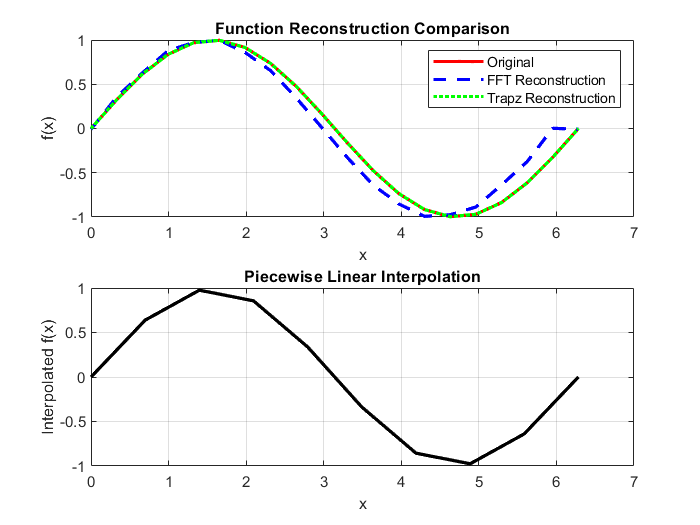
\includegraphics[width=0.75\linewidth]{Fourier Approximation//Fourier Analysis/fourieranalysis1.png}
        \label{fig:enter-label}
    \end{figure}
    \item Display the Fourier coefficients \( a_k \) and \( b_k \) obtained from both methods.
    \begin{figure}[H]
        \centering
        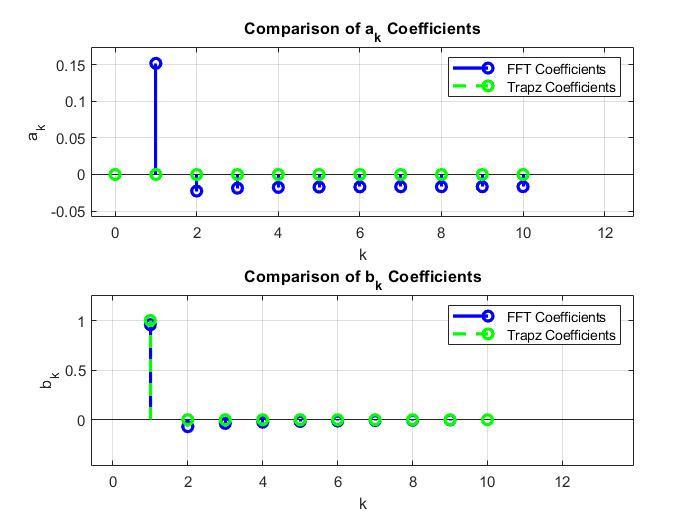
\includegraphics[width=0.75\linewidth]{Fourier Approximation//Fourier Analysis/fourieranalysis2.png}
        \label{fig:enter-label}
    \end{figure}
\end{itemize}

\dotfill

\noindent A similar piecewise linear interpolation can be done manually but it is a very tedious process. For example, take the function  $sin^2 x$ with 3 points including ends (done in my notes). We have the coefficients $b_k$ = 0 and 
\[
a_k = 
\begin{cases} 
\frac{-4}\pi k^2 & \text{k is odd}\\
0 & \text{k is even} \\
\end{cases}
\]
So, here $S_n (x)$ = $\Sigma_{k = 0}^n$ $a_k$ $cos(kx)$ with calculated $a_k$ as shown.\\\\
$\lvert f(x) - sin^2(x) \rvert$ = $\frac{1}{(n+1)^2}$ + $\frac{1}{(n+1)^2}$ + $\ldots$\\\\


\hl{(there's some proof about how the summation is is bounded or something, idk; then its extended to piecewise linear interpolation for  general function, just writing out in therms of variabes basically)}

\subsection{Analytical Proof}

\noindent\fbox{%
\parbox{\textwidth}{%
The sine and cosine functions are orthogonal over the interval \( [0, 2\pi] \). This property is fundamental in Fourier series analysis. The orthogonality conditions are defined as follows:

\begin{itemize}
    \item \textbf{Orthogonality of Sine Functions:}
    \[
    \int_{0}^{2\pi} \sin(mx) \sin(nx) \, dx =
    \begin{cases}
        0, & \text{for } m \neq n \\
        \pi, & \text{for } m = n \neq 0
    \end{cases}
    \]

    \item \textbf{Orthogonality of Cosine Functions:}
    \[
    \int_{0}^{2\pi} \cos(mx) \cos(nx) \, dx =
    \begin{cases}
        0, & \text{for } m \neq n \\
        \pi, & \text{for } m = n \neq 0 \\
        2\pi, & \text{for } m = n = 0
    \end{cases}
    \]

    \item \textbf{Orthogonality Between Sine and Cosine:}
    \[
    \int_{0}^{2\pi} \sin(mx) \cos(nx) \, dx = 0, \quad \text{for any } m, n.
    \]
\end{itemize}

These properties mean that when integrating the product of two different sine or cosine functions over a full period \( [0, 2\pi] \), the result is zero. This orthogonality is crucial for expressing periodic functions as a sum of sine and cosine terms in a Fourier series.
}%
}

\hl{proof that Sn(x) goes to zero if n tends to infinity, Sn(x) tends to f(x), }

\section{Collocation using Fourier Series as Basis}
$S_n(x)$ is the approximation for the function f(x) using its Fourier series representation. The collocation points are $x_k$. The Fourier series decomposes a periodic function into a sum of sine and cosine terms as 
\[
    S_n (x) = \alpha_0 + \sum_{m=1}^{\infty} \left( \alpha_m \cos\left(\frac{2 \pi m x}{T}\right) + \beta_m \sin\left(\frac{2 \pi m x}{T}\right) \right)   
\]
and
\[
S_n (x_k) = f (x_k) 
\]
with $x_k$ = $\frac{T k}{2n}$ for k = 0, 1, 2, $\ldots$ 2n+1\\\\
Using relations \ref{eq:fourier_ak} and \ref{eq:fourier_bk}, where dx = $\frac{T}{2n+1}$ 
\[
 \alpha_m = \frac{2}{2n+1} \sum^{2n+1}_{k=1} f(x_k) \cos\left(\frac{2 \pi m x}{T}\right) 
\]
\[
 \beta_m =  \frac{2}{2n+1} \sum^{2n+1}_{k=1} f(x_k)  \sin\left(\frac{2 \pi m x}{T}\right)
\]

\subsection*{Example: Fourier Series Approximation of (\href{https://github.com/abhx7/PseudoSpectral-Methods-in-Optimal-Control/blob/main/Codes/fourier_interpolation_sincos_triangle_wave.m}{Numerical})}
We approximate a given piecewise function \( f(x) \) using its Fourier series representation. A periodic function \( f(x) \) defined over the interval \( [0, 2\pi] \) can be approximated by a Fourier series.
\begin{itemize}
    \item \textbf{Initialization and Sample Points:}
    \begin{itemize}
        \item The number of terms in the series \( n \) is set.
        \item The vector \( x \) represents the points sampled from the interval \( [0, 2\pi] \), specifically \( 2n + 1 \) points for better accuracy.
    \end{itemize}
    
    \item \textbf{Definition of the Function:}
    \begin{itemize}
        \item The piecewise function is defined as:
        \[
        f(x) = 
        \begin{cases} 
        \frac{x}{\pi}, & \text{for } 0 \leq x < \pi, \\
        2 - \frac{x}{\pi}, & \text{for } \pi \leq x \leq 2\pi.
        \end{cases}
        \]
        \item This is represented as two segments, \( \texttt{fx1} \) for \( [0, \pi] \) and \( \texttt{fx2} \) for \( [\pi, 2\pi] \).
    \end{itemize}
    
    \item \textbf{Calculation of Coefficients:}
    The Fourier coefficients \( \alpha_m \) and \( \beta_m \) using numerical integration (via the \texttt{trapz} function) as shown above for a specific piecewise function defined over the interval \( [0, 2\pi] \). 
        % \item The coefficient \( a_0 \) (the DC component) is computed using the trapezoidal rule over the two intervals:
        % \[
        % a_0 = \frac{1}{\pi} \left( \int_{0}^{\pi} f(x) \, dx + \int_{\pi}^{2\pi} f(x) \, dx \right).
        % \]
        % \item For \( k \geq 1 \), the coefficients \( a_k \) and \( b_k \) are calculated similarly:
        % \[
        % a_k = \frac{1}{\pi} \left( \int_{0}^{\pi} f(x) \cos(kx) \, dx + \int_{\pi}^{2\pi} f(x) \cos(kx) \, dx \right),
        % \]
        % \[
        % b_k = \frac{1}{\pi} \left( \int_{0}^{\pi} f(x) \sin(kx) \, dx + \int_{\pi}^{2\pi} f(x) \sin(kx) \, dx \right).
        % \]
    
    \item \textbf{Function Reconstruction:}
    \begin{itemize}
        \item The function \( S_n(x) \) is reconstructed using the calculated \( \alpha_m \) and \( \beta_m \) coefficients.
        \item The approximation \( S_n(x) \) is then compared to the original piecewise function \( f(x) \) by calculating the squared error \( e(x) \).
    \end{itemize}
\end{itemize}

\subsubsection*{Plotting and Analysis}
\begin{itemize}
    \item The first plot displays the original function \( f(x) \) and its Fourier series approximation \( S_n(x) \).
    \begin{figure}[H]
        \centering
        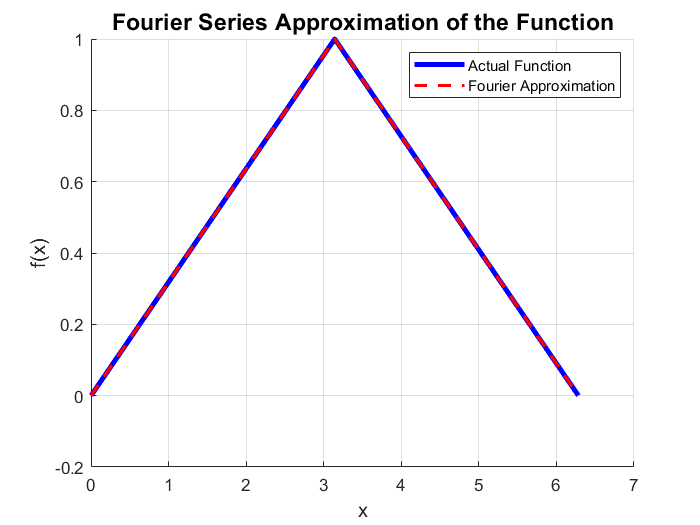
\includegraphics[width=0.75\linewidth]{Fourier Approximation//FourierBasisCollocation/fourierapprox.png}
        \label{fig:enter-label}
    \end{figure}
    \item The second plot visualizes the squared error \( e(x) \) across the interval, which helps to assess the quality of the approximation.
    \begin{figure}[H]
        \centering
        \includegraphics[width=0.75\linewidth]{Fourier Approximation//FourierBasisCollocation/error_fourierapprox.png}
        \label{fig:enter-label}
    \end{figure}
\end{itemize}
This numerical approach highlights the convergence behavior of the Fourier series in approximating piecewise continuous functions.



\end{document}
